\documentclass[aspectratio=169,12pt]{beamer}
\usepackage{fontspec}
\setsansfont{Arial}
\usepackage{tikz}
\usepackage{booktabs}
\usepackage{xurl}
\usetikzlibrary{arrows.meta,positioning}
\definecolor{ink}{HTML}{18303F}
\definecolor{teal}{HTML}{007F83}
\definecolor{muted}{HTML}{526371}
\definecolor{pale}{HTML}{EEF5F5}
\definecolor{warning}{HTML}{B04C35}
\setbeamercolor{normal text}{fg=ink,bg=white}
\setbeamercolor{frametitle}{fg=ink}
\setbeamercolor{structure}{fg=teal}
\setbeamercolor{alerted text}{fg=warning}
\setbeamerfont{frametitle}{size=\fontsize{22}{25}\selectfont,series=\bfseries}
\setbeamersize{text margin left=9mm,text margin right=9mm}
\setbeamertemplate{navigation symbols}{}
\setbeamertemplate{itemize items}{\small\color{teal}\textbullet}
\setbeamertemplate{frametitle}{\vspace{3mm}\insertframetitle\par\vspace{2mm}}
\setbeamertemplate{footline}{\hspace{9mm}\color{muted}\fontsize{6.5}{8}\selectfont Investify\quad FYP-1 Mid-Evaluation\hfill Fall 2026\quad Report date: 11 October 2026\quad\insertframenumber/\inserttotalframenumber\hspace{9mm}\vspace{3mm}}
\setbeameroption{hide notes}
\hypersetup{pdftitle={Investify FYP-1 Mid-1},pdfauthor={Investify project team},colorlinks=true,urlcolor=teal}
\newcommand{\source}[1]{\par\vspace{2mm}{\color{muted}\fontsize{6.5}{8}\selectfont Evidence: \nolinkurl{#1}\par}}
\newcommand{\lead}[1]{{\color{teal}\bfseries #1}\par\vspace{2mm}}
\tikzset{nodebox/.style={draw=teal,fill=pale,align=center,inner sep=2mm,font=\fontsize{10}{12}\selectfont},flow/.style={-{Stealth[length=2mm]},thick,draw=teal},plain/.style={align=left,font=\fontsize{10}{12}\selectfont}}
\begin{document}

\begin{frame}[plain]
\vspace{5mm}
{\color{teal}\large F26-003\quad FYP-1 Mid-Evaluation}\par\vspace{5mm}
{\fontsize{38}{42}\selectfont\bfseries Investify}\par\vspace{3mm}
{\Large Educational equity decisions\\with evidence and checked explanations}\par\vspace{7mm}
{\small Ahmed Javaid (22I-2530)\quad Rafay Ul Haq (22I-2520)\\Soban Ahmad (22I-2460)}\par\vspace{2mm}
{\small Supervisor: Mr. Irfan Ullah}\par\vspace{3mm}
{\color{muted}\footnotesize Fall 2026\quad Report date: 11 October 2026}
\note{Assigned presenter: Ahmed Javaid. Planned speaking: 30 seconds. Introduce the confirmed team and supervisor. This is FYP-1 Mid-Evaluation in Fall 2026. The team-selected report date is Sunday, 11 October 2026; the revision and tests retain their actual dates, including 12-13 October. The formal committee appointment is separate. The project is an educational prototype. It does not execute orders or establish investment suitability. The team delivered its assigned module parts and continues practice. Development assistance is disclosed in the report. Sources: report/main.tex and docs/team/MID1_TEAM_GUIDE.md.}
\end{frame}

\begin{frame}{Problem and research contribution}
\lead{Make decisions and explanations inspectable.}
\begin{itemize}\setlength{\itemsep}{3mm}
\item Temporal evaluation: use only information available at decision time.
\item Evidence: inspect technical/news values and raw-score contributions.
\item Checking: reject contradictory visible claims and verify recovery.
\end{itemize}
\vspace{3mm}{\small News/social divergence and user-comprehension evaluation remain later work.}
\note{Rafay, 60 seconds. Explain the implemented temporal and verification contributions; distinguish planned divergence and human outcomes.}
\end{frame}

\begin{frame}{Scope and acceptance checks}
\begin{columns}[T,onlytextwidth]\begin{column}{.48\textwidth}\lead{Current scope}\begin{itemize}\item Historical NVDA, five sessions\item Five technical + six news inputs\item Complete capacity/tolerance score\item Low-confidence abstention\end{itemize}\end{column}\begin{column}{.48\textwidth}\lead{Observable acceptance}\begin{itemize}\item Validate source/case identity\item Preserve model direction\item Reject wrong prose / JSON\item Check fallback independently\end{itemize}\end{column}\end{columns}
\note{Ahmed, 60 seconds. New multiclass records are separate from preserved isotonic failures. The full FYP and useful forecasting are distinct goals.}
\end{frame}

\begin{frame}{Mid-1 deliverables}
\small
\begin{tabular}{@{}p{.25\textwidth}p{.69\textwidth}@{}}\toprule\textbf{Area}&\textbf{Evidence}\\\midrule
Report & Detailed use cases, grouped requirements, metrics and individual tests\\[3mm]
Design & Six-module architecture, keys/cardinalities and behavioral models\\[3mm]
Live core & Evidence, eighteen-answer profile, uncertainty and checking/recovery\\[3mm]
Process & Member delivery, dated plan, Windows/Ubuntu CI and verified artifacts\\\bottomrule\end{tabular}\par
\vspace{4mm}{\small Supervisor checkpoint; planned presentation/demo duration: fifteen minutes.}
\note{Ahmed, 70 seconds. Connect the report artifacts to code. Hosted receipts prove their committed snapshots; current local source needs its matching new delivery.}
\end{frame}

\begin{frame}{System architecture}
\centering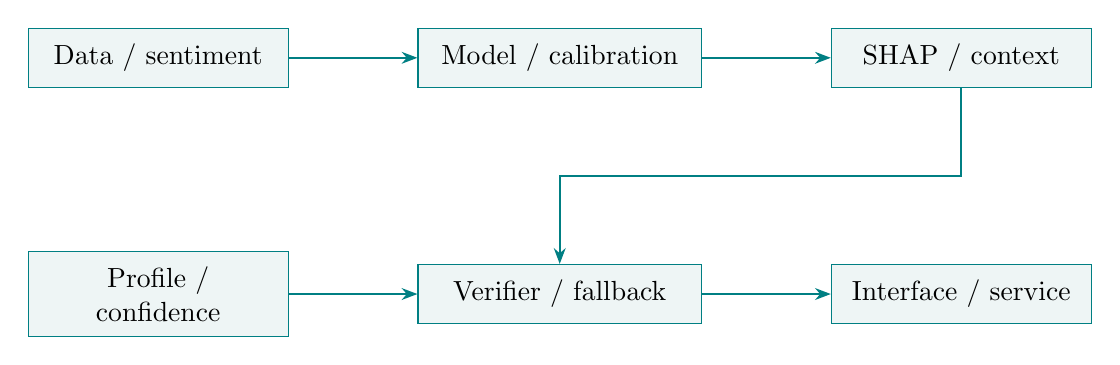
\begin{tikzpicture}[x=1mm,y=1mm]
\node[nodebox,text width=29mm] (data) at (17,40){Data / sentiment};\node[nodebox,text width=32mm] (model) at (68,40){Model / calibration};\node[nodebox,text width=29mm] (context) at (119,40){SHAP / context};
\node[nodebox,text width=29mm] (profile) at (17,10){Profile / confidence};\node[nodebox,text width=32mm] (guard) at (68,10){Verifier / fallback};\node[nodebox,text width=29mm] (ui) at (119,10){Interface / service};
\draw[flow](data)--(model);\draw[flow](model)--(context);\draw[flow](context.south)--(119,25)--(68,25)--(guard.north);\draw[flow](profile)--(guard);\draw[flow](guard)--(ui);
\end{tikzpicture}\par\vspace{3mm}{\small Model probabilities remain fixed during profile calculation and explanation checking.}
\note{Soban, 50 seconds. Describe the six product modules and the implemented historical slice. Social divergence, student serving and hosting remain later integrations.}
\end{frame}

\begin{frame}{Domain model and file schema}
\begin{itemize}\setlength{\itemsep}{3mm}\item Experiment identity: source + artifact digest\item Case identity: experiment + session\item Record: class, probabilities, feature/SHAP maps and model hashes\item Profile/candidate/result: local state with current identity binding\end{itemize}\vspace{3mm}{\small The report supplies attributes, keys and cardinalities. Storage uses file/session contracts; no SQL database is claimed.}
\note{Rafay, 60 seconds. Show the actual file and session relationships and explain why a changed case/profile invalidates the previous candidate result.}
\end{frame}

\begin{frame}{Explanation check and recovery}
\begin{enumerate}\setlength{\itemsep}{3mm}\item Read the current record and visible candidate.\item Verify prose and structured claims independently.\item Retain candidate rejection; construct deterministic fallback.\item Verify fallback, then show current output or an explicit error.\end{enumerate}\vspace{3mm}{\small Correct JSON cannot conceal an incorrect displayed probability.}
\note{Soban, 45 seconds. Trace emit and verify. The sequence/activity models include the click, alternative branches and fallback failure.}
\end{frame}

\begin{frame}{Live demonstration}
\begin{enumerate}\setlength{\itemsep}{3mm}\item \textbf{Decision}: diagnostic class/probabilities and uncertainty\item \textbf{Evidence}: technical and news feature meaning/effect\item \textbf{Risk}: published tolerance score, allowance and confidence requirement\item \textbf{Explanation}: inject 1.00\%, reject and verify fallback\end{enumerate}\vspace{3mm}{\small Multiclass frozen NVDA / 21 December 2023. Calculations/checking run live; model outputs are recorded.}
\note{Shared, 240 seconds: Rafay opens 20; Soban Decision 40; Ahmed Evidence 40; Rafay Risk 60; Soban Explanation 80. Both profile extremes abstain on weak real evidence; show the changing score/threshold without claiming fabricated prediction quality.}
\end{frame}

\begin{frame}{Calibration correction and abstention}
\begin{tabular}{@{}lrr@{}}\toprule\textbf{Frozen mode}&\textbf{Buy/Hold/Sell}&\textbf{Macro-F1}\\\midrule
Raw model & 40 / 51 / 95 & 0.3182\\[3mm]
Independent isotonic & 186 / 0 / 0 & 0.2238\\[3mm]
Global temperature & 40 / 51 / 95 & 0.3182\\\bottomrule\end{tabular}\par
\vspace{4mm}\lead{The correction preserves order, not useful signal.}
{\small Temperature reaches its upper bound; probabilities approach one-third. The interface withholds directional suggestions.}
\note{Soban, 55 seconds. Explain the isotonic global bounds, calibration-only temperature fit and why near-uniform confidence requires abstention. Do not describe this as useful forecasting.}
\end{frame}

\begin{frame}{Temporal leakage experiment}
\begin{tabular}{@{}lrr@{}}\toprule\textbf{Five-session arm}&\textbf{Macro-F1}&\textbf{Lift}\\\midrule
Clean & 0.2843 & -0.0444\\[3mm]
Shuffled & 0.4457 & +0.1142\\[3mm]
Centred Bollinger & 0.5390 & +0.2104\\\bottomrule\end{tabular}\par
\vspace{4mm}{\small No-purge and same-bar variants do not guarantee inflation. Endpoint purge and the configured calendar-day gap are distinct controls.}
\note{Ahmed, 100 seconds. Explain actual label availability, how the canary fires, and why a weak no-purge/lag variation is not proof that every leakage mechanism is absent. State the FNSPID precision/coverage reason for the timestamped source.}
\end{frame}

\begin{frame}{Sentiment and teacher studies}
\begin{columns}[T,onlytextwidth]\begin{column}{.48\textwidth}\lead{Social comparison}{\small Same 24 held-out references}\par\vspace{3mm}\begin{tabular}{@{}lr@{}}\toprule Candidate&Macro-F1\\\midrule CryptoBERT&0.2564\\Cardiff&0.6016\\\bottomrule\end{tabular}\par\par\vspace{3mm}{\small Crypto probes return positive/negative; equity outputs remain all neutral.}\end{column}\begin{column}{.48\textwidth}\lead{Teacher construction}\begin{itemize}\item Actual recorded prose\item Deterministic factual targets\item Student remains untrained\item Larger comparison is later\end{itemize}\end{column}\end{columns}\vspace{3mm}{\small Small reference sample; independent validation and deployment selection remain open.}
\note{Rafay, 100 seconds. FinBERT still scores news. CryptoBERT/Cardiff are social candidates. Sanity probes are separate authored diagnostics, not benchmark accuracy. Teacher/student method is disclosed once in the report.}
\end{frame}

\begin{frame}{Delivered work and next milestones}
\small
\begin{tabular}{@{}p{.23\textwidth}p{.70\textwidth}@{}}\toprule\textbf{Member}&\textbf{Delivered part / continuation}\\\midrule Ahmed&Temporal data, leakage and CI/delivery; parity/deployment next\\[3mm]
Rafay&Interface, profile and sentiment; divergence/acceptance next\\[3mm]
Soban&Engine, calibration, SHAP and verifier; student/QLoRA next\\\bottomrule\end{tabular}\par\vspace{4mm}{\small One-third responsibility and five minutes each. Internal dated targets are in the report; current code practice continues.}
\note{Soban, 30 seconds. Confirm delivered responsibilities and shared allocation. Future research/hosting and participant work are distinct from this checkpoint.}
\end{frame}
\end{document}
